% !TEX root = thesis-ex.tex
Of the jet reconstruction algorithms that were discussed in Section~\ref{sec:jet_algo}, the LHC collaborations use the \antikt\ algorithm.
The ATLAS jet reconstruction procedure in heavy ion collisions is described in Ref.~\cite{2019108}, and is summarized in Figure~\ref{fig:atlasHIjetreco}.
It is different from the procedure for \pp\ collisions because of the large underlying event present in the heavy ion collision system.
%The heavy ion jet reconstruction procedure however, can also be applied to \pp\ collisions with ,

\begin{figure}[htbp!]
	\centering
	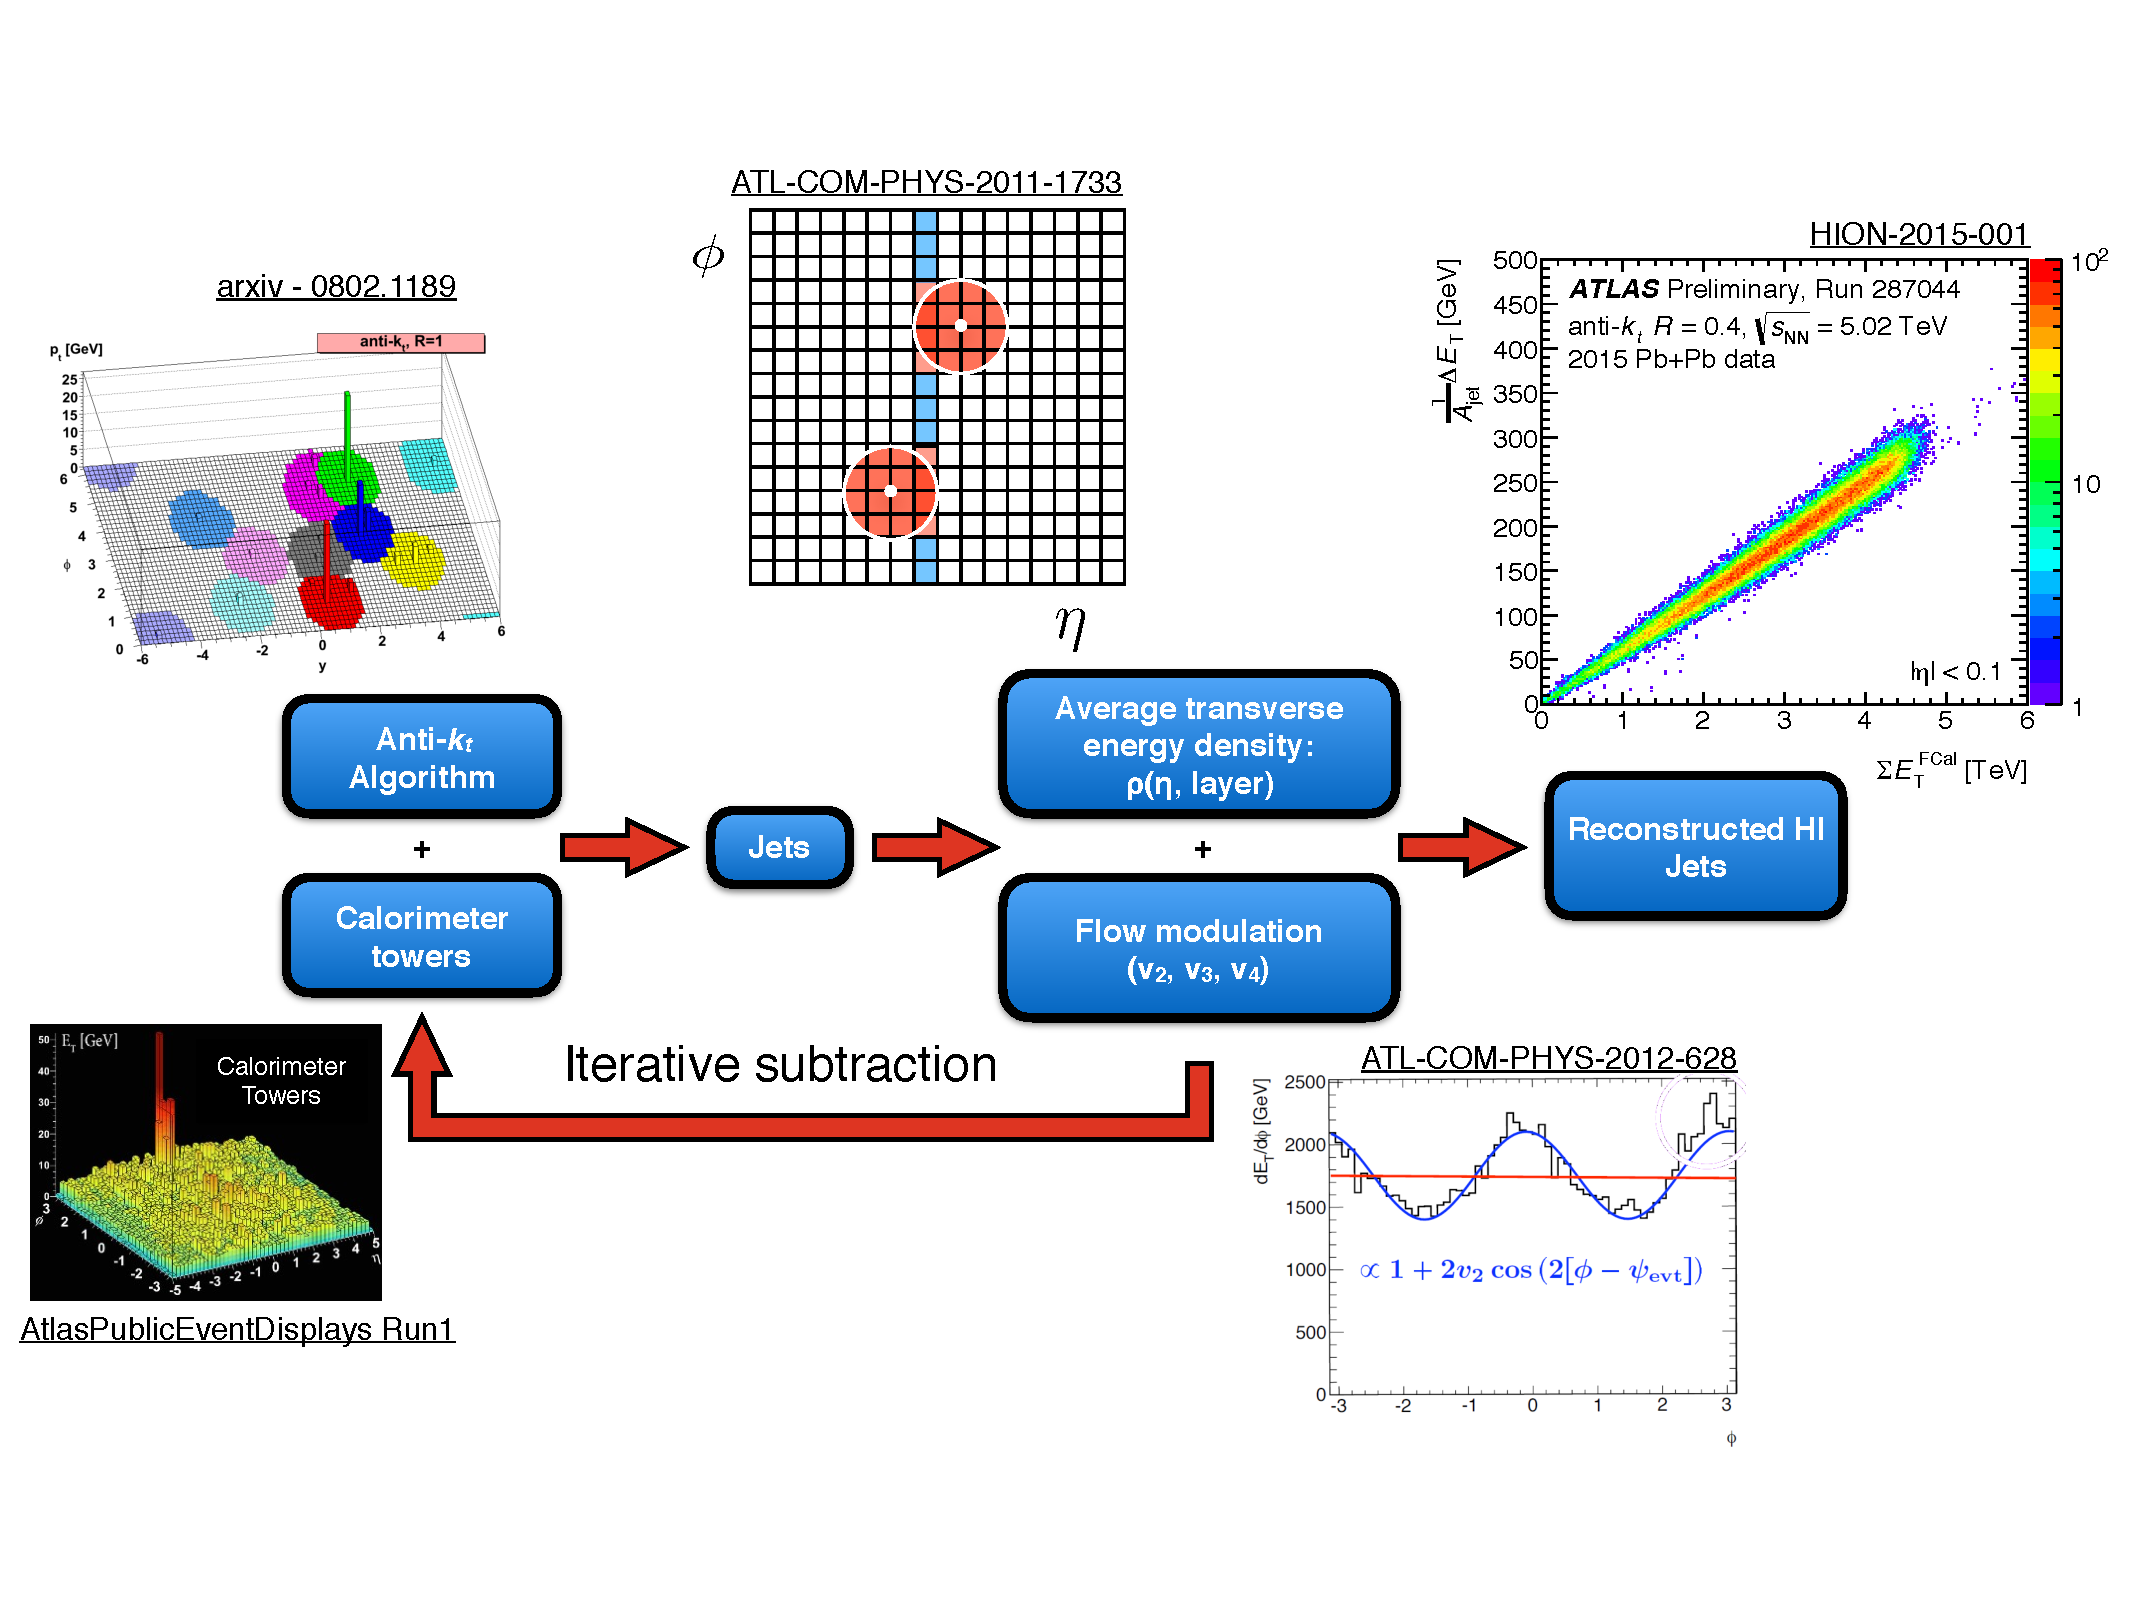
\includegraphics[width=\textwidth]{figures/setup/atlasHIjetReco} %
	\caption{A schematic of the ATLAS jet reconstruction procedure.
	Figures taken from \cite{Cacciari:2008gp, atlasRun1EventDisplay, ATLAS-COM-PHYS-2011-1733, Cole:1450219, perfPlots}.}	
	\label{fig:atlasHIjetreco}%
\end{figure}

This procedure uses the \antikt\ algorithm as implemented in \textsc{FastJet} software package \cite{fastjet_algo}.
The \antikt\ algorithm is run in four-momentum recombination mode with its inputs being the $\eta \times \phi = 0.1 \times \pi / 32$ calorimeter towers.
The tower energies are the sum of the energies of all layers in the tower with cells that straddle tower boundaries having their energies fractionally distributed.
The \antikt\ algorithm is first run with the distance parameter $R=0.2$, to give seed jets.

These seed jets contain at least one tower with $\Et > 3$ GeV, and have the ratio of the maximum tower transverse energy to the average tower transverse energy, $\Et^{Max} / \langle \Et \rangle > 4$.
Then the underlying event subtraction procedure is performed.
A first estimate of the average underlying event energy density $\rho_i (\eta)$ is done in 0.1 slices of $\eta$ in each calorimeter layer $i$ after excluding the regions that overlap with the seed jets.
A modulation is applied to account for the flow from the QGP (discussed in Section~\ref{sec:qgp}) and the underlying event is subtracted to give $E_{Tj}^{\mathrm{sub}}$:

\begin{align}
E_{Tj}^{\mathrm{sub}} = E_{Tj} - A_j \rho_i (\eta_j) \Big(1+2 \sum_{n=2}^{4} {v_{n}}_i \big(\cos[2(\phi_j-\Psi_n)] \big) \Big)
\end{align}
where $E_{Tj} , \eta_j, \phi_j$ and $A_j$ are the cell $E_T, \eta, \phi$ and area for cell $j$ in layer $i$.
$v_{ni}$ are the $n^{\rm th}$ order harmonics of the modulation in layer $i$and are given by:

\begin{align}
v_{ni} = \frac{\sum_{j \in i} \Et_j \cos[2(\phi_j-\Psi_n)]}{\sum_{j \in i} \Et_j}
\end{align}
where the sum is over all cells $j$ in layer $i$.
$\Psi_n$ is the event plane angle and is given by \cite{ATLAS:2012at}:

\begin{align}
\Psi_n = \frac{1}{n} \tan^{-1} \left[ \frac{\langle \sum_k w_k \Et_k \sin(n\phi_k) \rangle}{\sum_k \Et_k \sin(n\phi_k)} \right]
\end{align}
where the sum is over all $k$ cells in the FCal and $\phi_k$ is the azimuthal angle of the cell.
The $w_k$ weights are to ensure a uniform $\Psi_n$ distribution.
The dominant effect in the modulation is from the second and third harmonic, $v_2$ and $v_3$ \cite{ATLAS:2012at}.

Once the background is subtracted, the \antikt\ algorithm is run again with the distance parameter $R = 0.2$.
The underlying event is re-estimated after excluding areas that are within $\Delta R = 0.4$ of the seeds.
Updated values of $\rho{'}_i$ and $v{'}_2$ are recalculated and used to estimate the background that is subtracted from the original cell energies.
This is then subtracted from the original cell energies to give kinematics for the $R= 0.4$ jets.
The average subtracted energy normalized by the area of the jet reconstructed jet, as a function of the energy in the forward calorimeter is shown in Fig~\ref{fig:subtr_energy}.
It can be seen that in the barrel region for $|\eta| < 0.1$, $R=0.4$ jets have a background that is approximately $300/(\pi\times 0.4^2) \approx 150$ GeV.

\begin{figure}[htbp!]
	\centering
	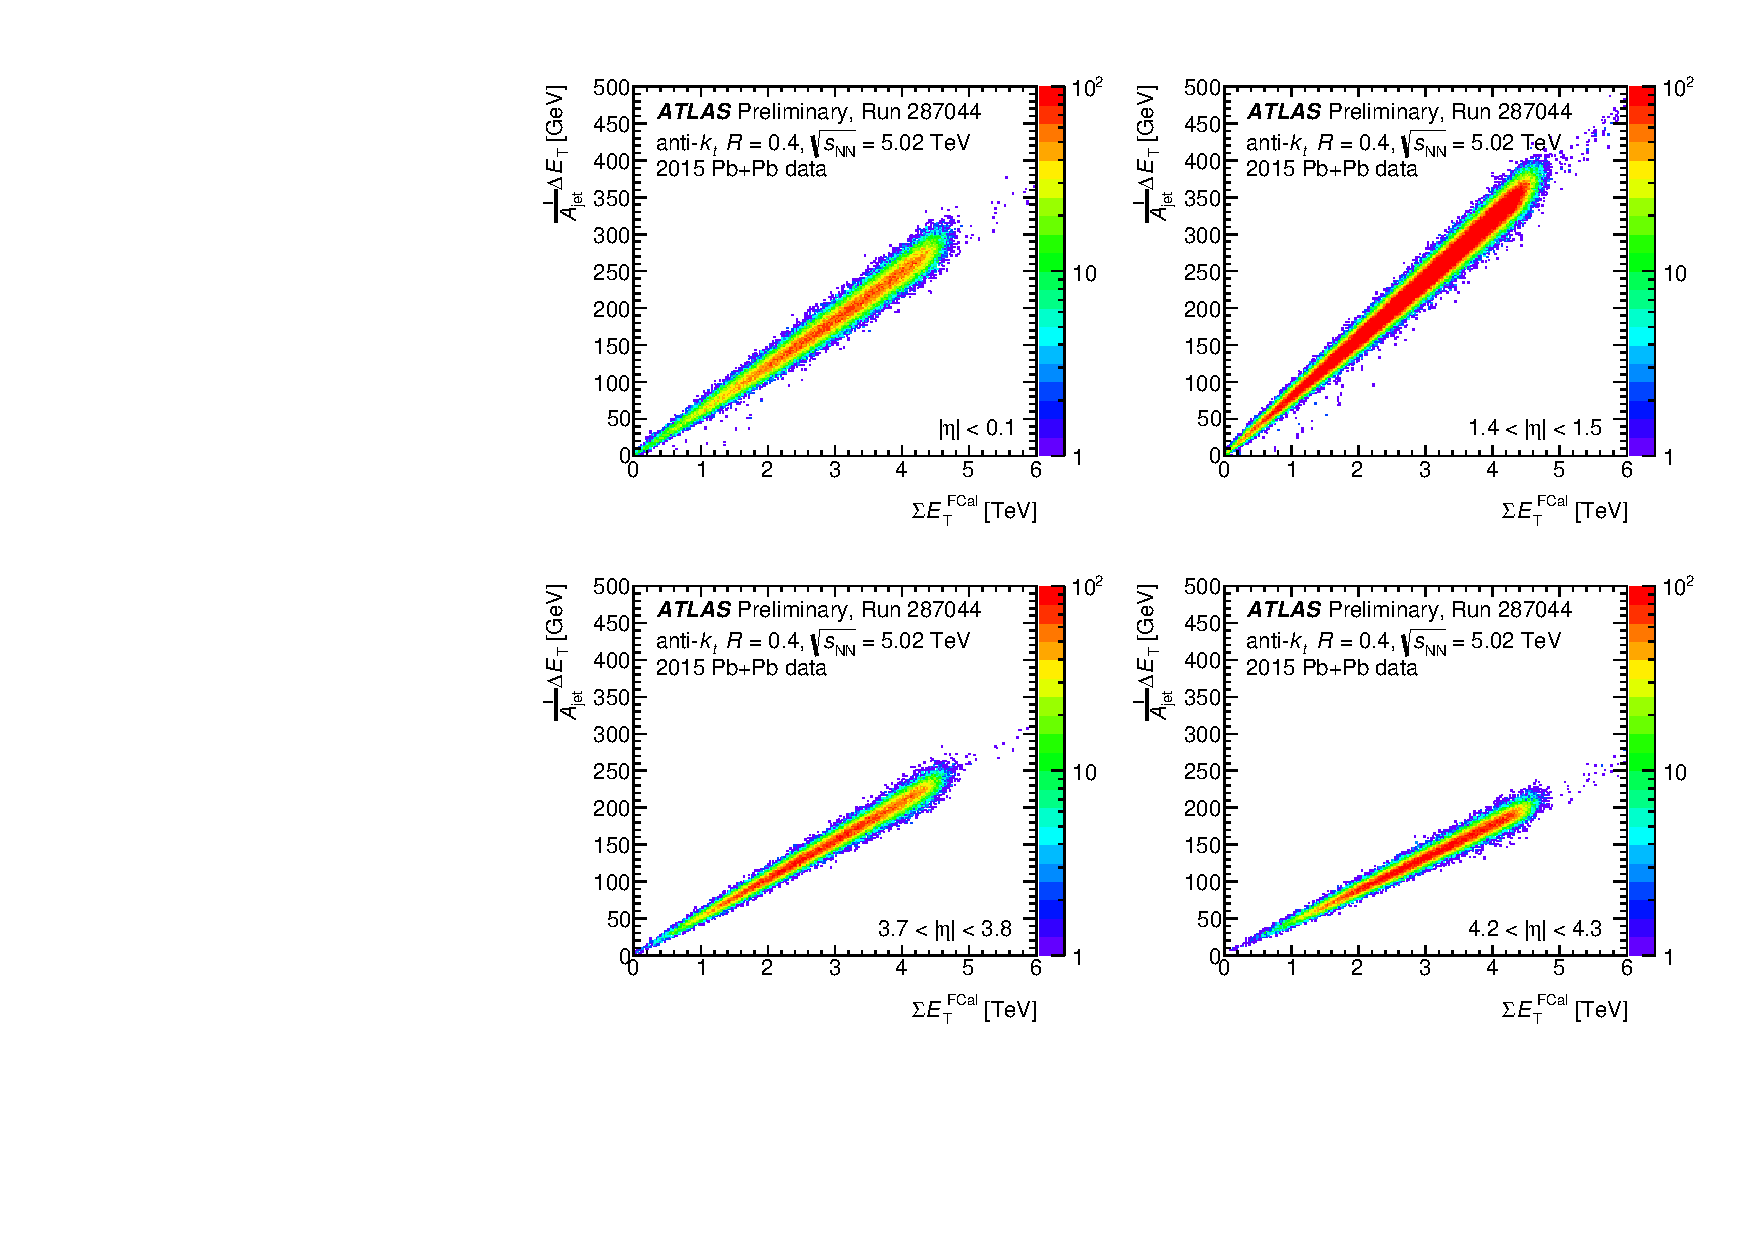
\includegraphics[width=0.6\textwidth]{figures/setup/subtr_energy} %
	\caption{
	The subtracted transverse energy $\Delta \Et$, normalized by the area of the jet $A_{\rm{jet}}$ as a function of the sum of the energy deposited in the forward calorimeter $\sum \Et_{\rm FCal}$ in \pbpb\ collisions at $\sqrtsnn = 5.02$ TeV.
	The jets were reconstructed using the \antikt\ algorithm with $R = 0.4$.
	Four panels show four selections on the pseudorapidity of the jet.
	Figures taken from \cite{perfPlots}.}	
	\label{fig:subtr_energy}
\end{figure}


These jets still require a calibration before they can be used for analysis.
This includes the following \cite{Aad:2014bia}:
\subparagraph{Origin Correction: } This correction ensures that jets point back to the primary vertex and not the nominal center of the detector.
\subparagraph{MC based Calibration: } This is a MC based correction that depends on the comparison between the energy and pseudorapidity of the reconstructed jet and the corresponding matched truth jet.
\subparagraph{\textit{In situ}+Cross Calibration: } This calibration is based on the differences between data and MC as described by a well-measured object like a photon or Z boson.
This poses a challenge for heavy ion collisions because unlike in \pp\ collisions, there simply aren't enough statistics for these objects.
Here the cross-calibration procedure accounts for differences in the jet reconstruction procedure in heavy ion collisions and \pp\ collisions, and enables the usage of the \insitu\ corrections from \pp\ collisions.


The validity of the jet reconstruction and calibration procedure can be tested by evaluating the jet energy scale and jet energy resolution.
These are the mean and width respectively of the jet response distribution that is given by $\ptreco / \pttruth$ in MC and are shown in Figure~\ref{fig:jes_jer}.
\ptreco\ is the reconstructed jets transverse momentum, while \pttruth\ is the transverse momentum of the corresponding ``truth'' jet.


\begin{figure}[htbp!]
	\centering
	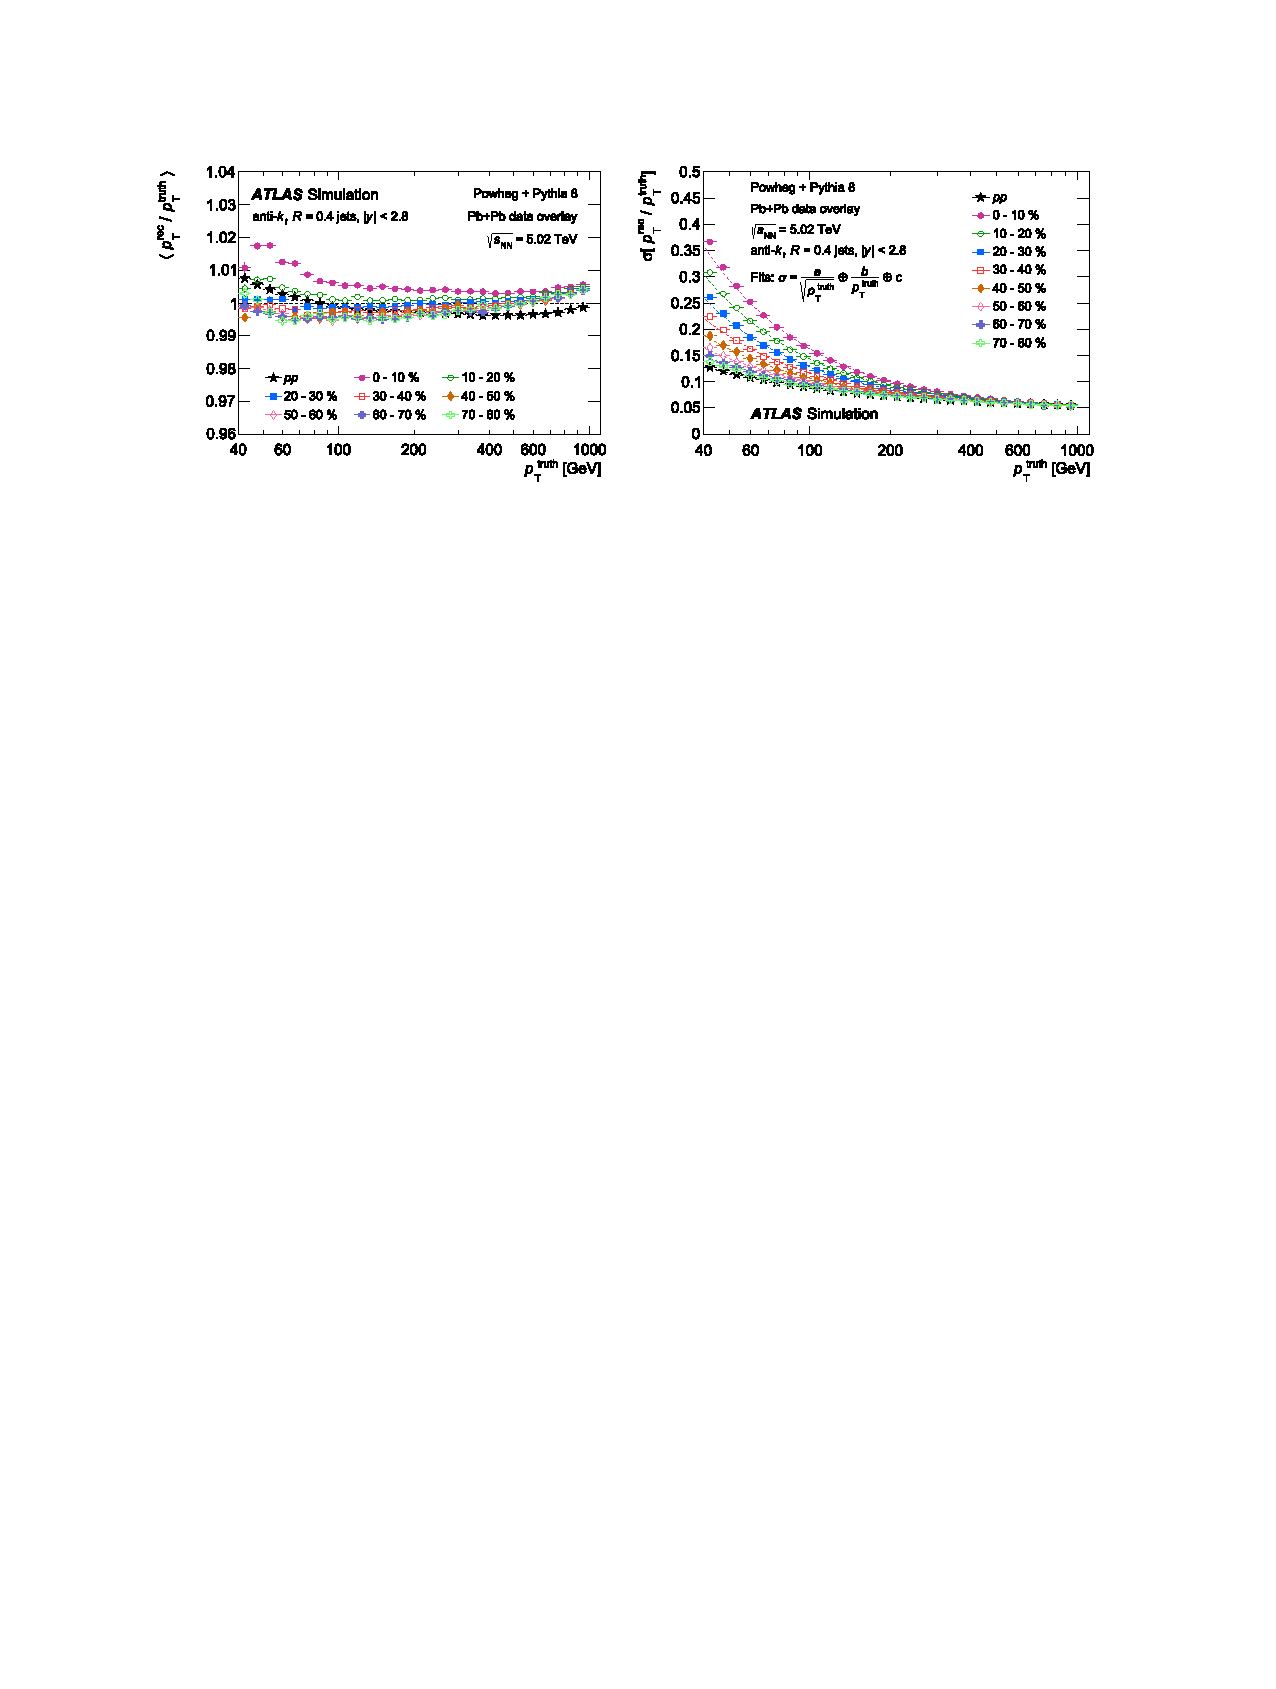
\includegraphics[width=\textwidth]{figures/setup/jes_jer} %
	\caption{
	The Jet Energy Scale (left) and Jet Energy Resolution (right) as a function of \pttruth.
	Both are for jets with $|y| < 2.8$. The different curves are for \pp\ and varying \pbpb\ centrality.
	Figures taken from \cite{2019108}.}	
	\label{fig:jes_jer}%
\end{figure}
The JES is seen to be almost unity within 1\%. across a broad kinematic range.
The JER is smaller for jets with higher transverse momentum, and depends on centrality.
It is the largest in central collisions and gets better for more peripheral collisions.
The JER can be fit to the form \cite{Aad:hi_jets}:

\begin{align}
\frac{\sigma[\Delta \Et]}{E_{\rm T}^{\rm true}} = \frac{a}{\sqrt{E_{\rm T}^{\rm true}}} \oplus \frac{b}{E_{\rm T}^{\rm true}} \oplus c
\end{align}
where $a$ and $c$ are related to the detector response.
The $b$ term describes the underlying event fluctuations and depends on centrality.
The large underlying event in central collisions results in the JER being the largest in that centrality interval. 
